\section{Tuesday, June 11}

\todaybox{We are going to continue discussing the Cauchy Integral theorem and primitives. This will necessitate we talk about path independence.}

Last time, we proved two fairly powerful theorems for integrating: our $\C$FTC and a version of the Cauchy Integral Theorem. I'd like to offer an alternative proof of the CIT:

\begin{ex}{}{} Consider this argument:

\begin{proof}Let $F$ be a primitive for $f$ on the open set $U$. Then by $\C$FTC:
$$\int_{\gamma} f(z)dz = F(\gamma(b)) - F(\gamma(a))$$

However, we know that $\gamma$ is closed, so $\gamma(a) = \gamma(b)$. As such:
$$\int_{\gamma} f(z)dz = F(\gamma(b)) - F(\gamma(b)) = 0$$\end{proof}

What's wrong with this proof? Why did we have to break out Green's theorem instead?

Well, this is predicated on us having a primitive $F$ for $f$! We don't know that analytic functions have primitives on any open set, and it turns out not to be true.
\end{ex}

So when does an analytic function have a primitive? How might we go about finding this function? For inspiration, we turn to a similar result from first year calculus, the Fundamental Theorem of Calculus.

Recall that the FTC has two parts. The first part we already have an analogue for, which is our $\C$FTC. The second part says that if $f(x)$ is a continuous function on $[a,b]$, then:
$$F(x) = \int_a^xf(t)dt$$

\noin is a differentiable function on $(a,b)$ with $F'(x) = f(x)$. I.e., that $F$ is an antiderivative for $f$.

If we try to emulate this definition in $\C$, we could try to define a function $F(z)$ on a domain $D$ as follows. Fix a point $z_0$ in $D$. For any point $z\in D$, we define
$$F(z) = \int_{\gamma_z}f(w)dw$$

\noin where $\gamma_z$ is any curve from $z_0$ to $z$ in $D$. Does this definition make sense? Well, we can compute these integrals for sure. So let's work out an example.

\begin{ex}{}{} Let $D = \C\setminus\{0\}$, and $f(z) = \frac{1}{z}$. This function is analytic on the domain $D$. We'll fix our point $z_0 =1$. Let's consider what this formula gives $F(-1)$. We will compute the integral along two curves:

\begin{center}
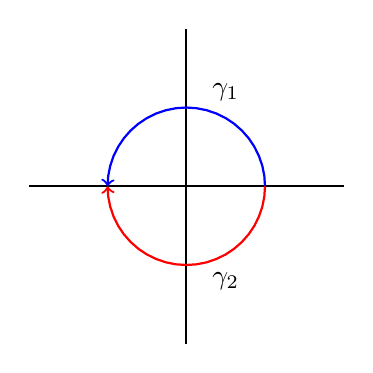
\begin{tikzpicture}
%\draw [help lines,black!20!white] (-1,-1) grid (4,4);

\draw[thick] (0,-2) -- (0,2);
\draw[thick] (-2,0) -- (2,0);

\draw [blue,thick,domain= 0:180, ->] plot ({cos(\x)}, {sin(\x)});
\draw [red,thick,domain= 180:360, <-] plot ({cos(\x)}, {sin(\x)});
\draw (0.5,-1.2) node {$\gamma_2$};
\draw (0.5,1.2) node {$\gamma_1$};

\end{tikzpicture}
\end{center}

The curve $\gamma_1$ is the upper semicircle of radius $1$ centered at $0$, travelled from $1$ to $-1$. We can parametrize it as $\gamma_1(t) = e^{it}$ for $t\in[0,\pi]$. Its derivative is $\gamma_1'(t) = ie^{it}$. So we compute the integral:
$$\int_{\gamma_1}\frac{1}{z}dz = \int_{0}^\pi \frac{1}{e^{it}}ie^{it}dt = \int_0^\pi idt = i\pi$$


The curve $\gamma_2$ is the lower semicircle of radius $1$ centered at $0$, travelled from $1$ to $-1$. We can parametrize it as $\gamma_2(t) = e^{-it}$ for $t\in[0,\pi]$. Its derivative is $\gamma_2'(t) = -ie^{it}$. So we compute the integral:
$$\int_{\gamma_2}\frac{1}{z}dz = \int_{0}^\pi -\frac{1}{e^{-it}}ie^{-it}dt = \int_0^\pi -idt = -i\pi$$

We find that $-i\pi = F(-1) = i\pi$, which tells us that $F$ isn't a function!
\end{ex}

In this example, we ran afoul of something very unfortunate: complex line integration is not path independent in general.

\subsection{Path Independence}

Let's investigate path independence of integrals. When can we guarantee that $\int_{\gamma_1}f(z)dz = \int_{\gamma_2}f(z)dz$? To begin, let's investiage this equation a bit more. If these integrals are equal, then we can rearrange to get:

\begin{align*}0 &= \int_{\gamma_1} f(z)dz - \int_{\gamma_2}f(z)dz\\
&= \int_{\gamma_1} f(z)dz + \int_{-\gamma_2} f(z)dz \hspace{50pt} \text{From week 5 homework, Q6}\\
&= \int_{\gamma_1 + (-\gamma_2)}f(z)dz \hspace{95pt}\text{From week 5 homework, Q7}
\end{align*}

So, the integrals $\int_{\gamma_1}f(z)dz$ and $\int_{\gamma_2}f(z)dz$ are equal if and only if the integral $\int_{\gamma_1 - \gamma_2}f(z)dz$, over the closed curve $\gamma_1 + (-\gamma_2)$ is $0$. This looks an awful lot like a Cauchy Integral Theorem type result. However, we have no guarantees that $\gamma_1 + (-\gamma_2)$ is smooth or simple. We only know that it is piecewise smooth and closed.

So, for the moment, let's try to generalize the Cauchy-Integral theorem to handle piecewise smooth, closed curves. To do so, we need to overcome several hurdles. We need to:

\begin{itemize}
\item define integration over piecewise smooth curves
\item show we can generalize CIT to handle piecewise smooth curves
\item show we can generalize CIT to handle non-simple closed curves
\end{itemize}

So, to begin, we define:

\begin{defbo}{}{}\index{Integral!piecewise smooth curve}Let $\gamma$ be a piecewise smooth curve. Then $\gamma$ can be written as $\gamma = \gamma_1 + \gamma_2 + \dots + \gamma_n$, where each $\gamma_j$ is a smooth curve.

We define the integral $\int_{\gamma}f(z)dz$ as:
$$\int_{\gamma}f(z)dz = \sum_{j = 1}^n \int_{\gamma_j}f(z)dz$$
\end{defbo}

Now, fortunately, extending CIT to work over piecewise smooth curves takes no work. Green's theorem applies to piecewise smooth, simple, closed curves as well.

To handle the closed case, the idea is fairly simple. If we have a closed curve, such as:

\begin{center}
\begin{tikzpicture}
\draw[fill = lightgray] (0,0) to[out = 0, in = 270] (1,1) to[out = 90, in = 45] (0,0);
\draw[fill = DEFinner] (-1,0.4) to [out = 0, in = 225] (0,0) to[out = 225, in = 260] (-1,0.4);
\draw[fill = CORinner] (-1.5,-2) to[out =70 , in = 240] (-1,0.4) to[out = 100, in = 30] (-2,-1) to[out = 30, in = 70] (-1.5,-2);

\end{tikzpicture}
\end{center}

\noin which is composed of three different piecewise smooth, closed curves. If $f$ is analytic on a domain containing each of these curves and their insides, then we can use CIT on each of them. Then the total integral will be the sum of each of these integrals, which will be $0$.

A complete proof of this is much more technical. So our proof will be somewhat "hand-wavey".

\begin{thmbo}{Cauchy's Integral Theorem (version 2)}{CIT2}\index{Cauchy's Integral Theorem!version 2} Let $f$ be a function that is analytic on a domain $D$. Suppose that $\gamma$ is a closed, piecewise smooth curve such that $D$ contains $\gamma$ and all of the regions bounded by $\gamma$. Then:
$$\int_{\gamma}f(z)dz = 0$$
\end{thmbo}

\begin{proof} The conditions on $\gamma$ ensure that $\gamma$ can be decomposed into:

\begin{itemize} 
\item countably many piecewise smooth, simple closed curves
\item countably many curves $\sigma_j$ such that $\gamma$ traverses each $\sigma_j$ an equal number in both directions
\end{itemize}

As such, we have that:

\begin{align*}\int_{\gamma}f(z)dz =& \sum_{\gamma_j \text{ is a simple, closed summand of} \gamma} \int_{\gamma_j}f(z)dz \\&+ \sum_{\sigma_j \text{ is a curve such that $\gamma$ traverses $\sigma_j$ an equal number of times in each direction}} n\left(\int_{\sigma_j} f(z)dz + \int_{-\sigma_j}f(z)dz\right)
\end{align*}

By our original CIT, the first summand is $0$. And since $\int_{\sigma_j}f(z)dz + \int_{-\sigma_j}f(z)dz = 0$, the second summand is $0$. Therefore:
$$\int_{\gamma}f(z)dz = 0$$

\end{proof}

We can use this to give one condition on path independence:

\begin{thmbo}{}{pathind} Suppose $f(z)$ is analytic on a domain $D$ containing the two curves $\gamma_1,\gamma_2$, which start and end at the same point, and which contains all points bounded between $\gamma_1,\gamma_2$. Then:
$$\int_{\gamma_1}f(z)dz = \int_{\gamma_2}f(z)dz$$
\end{thmbo}

\begin{proof} By CIT version 2:
$$\int_{\gamma_1 - \gamma_2}f(z)dz = 0$$

We showed earlier that this is equivalent to $\int_{\gamma_1}f(z)dz  =\int_{\gamma_2}f(z)dz$.
\end{proof}

